\documentclass[12pt,fleqn]{article}
\usepackage{amsfonts}
\usepackage{amsmath,amsthm,amssymb,graphicx,setspace,url,booktabs,tabularx,enumerate,slantsc}
\usepackage[T1]{fontenc}

\usepackage[sort,round,comma]{natbib}
\usepackage[margin=1.25in]{geometry}
\usepackage[small]{caption}
\usepackage[charter]{mathdesign}
\urlstyle{same}
\newcolumntype{C}{>{\centering\arraybackslash}X}
\bibliographystyle{abbrvnat}
\newcommand\citepos[2][]{\citeauthor{#2}'s \citeyearpar[#1]{#2}}
\newcommand\poscw{\citeauthor{ClW:06}'s \citeyearpar{ClW:06,ClW:07}}
\newcommand\citen[1]{\citeauthor{#1}, \citeyear{#1}}
\frenchspacing
\newcommand{\empiricalcriticalvalue}{2.67}
\newcommand{\spacriticalvalue}{1.26}
\newcommand{\nboot}{599}
\newcommand{\bootsize}{10}
\newcommand{\windowlength}{10}
\newcommand{\empiricaltable}{% latex table generated in R 3.2.0 by xtable 1.7-4 package
% Mon Apr 20 13:17:43 2015
\begin{tabularx}{\textwidth}{lCCCC}
  \toprule   & value & naive & SPA & ours \\ 
  \midrule long term rate & $\enskip1.56$ & sig. & sig. &  \\ 
  book to market & $\enskip1.41$ & sig. & sig. &  \\ 
  dividend yield & $\enskip1.27$ &  & sig. &  \\ 
  dividend price ratio & $\enskip0.95$ &  &  &  \\ 
  net equity & $\enskip0.70$ &  &  &  \\ 
  dividend payout ratio & $\enskip0.64$ &  &  &  \\ 
  treasury bill & $\enskip0.53$ &  &  &  \\ 
  stock variance & $\enskip0.50$ &  &  &  \\ 
  default return spread & $\enskip0.16$ &  &  &  \\ 
  default yield spread & $\enskip0.09$ &  &  &  \\ 
  inflation & $\!\!-0.09$ &  &  &  \\ 
  term spread & $\!\!-0.43$ &  &  &  \\ 
  earnings price ratio & $\!\!-0.56$ &  &  &  \\ 
  long term yield & $\!\!-0.74$ &  &  &  \\ 
   \bottomrule \end{tabularx}
}


% These commands are generated when the monte carlo and applied
% sections are run; I'm giving them definitions now so that LaTeX will
% run.
\providecommand\bootsize{[missing]}
\providecommand\empiricalcriticalvalue{[missing]}
\providecommand\nboot{[missing]}
\providecommand\testsize{[missing]}
\providecommand\totalsims{[missing]}
\providecommand\windowlength{[missing]}
\providecommand\empiricaltable{[missing]}

\newtheorem{thm}{Theorem}
\newtheorem{lem}[thm]{Lemma}
\newtheorem{claim}[thm]{Claim}
\newtheorem{cor}[thm]{Corollary}
\newtheorem{lema}{Lemma}[subsection]
\newtheorem{alg}{Algorithm}
\newtheorem{asmp}{Assumption}
\theoremstyle{definition}

\newtheorem{example}{Example}
\newtheorem{defn}{Definition}
\newtheorem{rem}{Remark}

\DeclareMathOperator*{\argmin}{arg\,min}
\DeclareMathOperator{\E}{E}
\DeclareMathOperator{\var}{var}
\DeclareMathOperator{\cov}{cov}
%\DeclareMathOperator{\vec}{vec}
\DeclareMathOperator{\vech}{vech}

\DeclareMathOperator{\pr}{Pr}

\newcommand{\btrue}{\beta_0}

\newcommand{\X}{\ensuremath{\mathrm{X}}}
\newcommand{\R}{\ensuremath{\mathrm{R}}}
\newcommand{\p}{\ensuremath{\mathrm{P}}}

\newcommand{\bh}{\hat \beta}
\newcommand{\ep}{\varepsilon}
\newcommand{\eph}{\hat\varepsilon}
\newcommand{\fb}{\bar f}
\newcommand{\fh}{\hat f}
\newcommand{\Hs}{\mathcal{H}}

\newcommand{\osum}[1]{\sum_{#1=R}^{T-1}}
\newcommand{\omax}[1]{\max_{#1=R,\dots,T-1}}
\newcommand{\oavg}[1]{\tfrac{1}{P} \osum{#1}}
\newcommand{\oclt}[1]{\tfrac{1}{\sqrt{P}} \osum{#1}}

\newcommand{\aic}{AIC}
\newcommand{\bic}{BIC}
\newcommand{\brc}{BRC}
\newcommand{\cdf}{CDF}
\newcommand{\clt}{CLT}
\newcommand{\dd}[1]{\frac{\partial}{\partial #1}}
\newcommand{\dgp}{DGP}
\newcommand{\fclt}{FCLT}
\newcommand{\fwe}{FWE}
\newcommand{\gdp}{GDP}
\newcommand{\gmm}{GMM}
\newcommand{\hac}{HAC}
\newcommand{\iv}{IV}
\newcommand{\lln}{LLN}
\newcommand{\ma}{MA}
\newcommand{\mds}{MDS}
\newcommand{\ned}{NED}
\newcommand{\ols}{OLS}
\newcommand{\oos}{OOS}
\newcommand{\sfwe}{SFWE}
\newcommand{\spa}{SPA}
\newcommand{\wfwe}{WFWE}

\renewcommand{\Re}{\ensuremath{\mathbb{R}}}

\renewcommand{\topfraction}{.85}
\renewcommand{\bottomfraction}{.7}
\renewcommand{\textfraction}{.15}
\renewcommand{\floatpagefraction}{.66}
\renewcommand{\dbltopfraction}{.66}
\renewcommand{\dblfloatpagefraction}{.66}
\setcounter{topnumber}{9}
\setcounter{bottomnumber}{9}
\setcounter{totalnumber}{20}
\setcounter{dbltopnumber}{9}

\begin{document}

\author{Gray Calhoun\thanks{Economics Department; Iowa State
    University; Ames, IA 50011.  Telephone: (515) 294-6271.  Email:
    \guillemotleft\protect\url{gcalhoun@iastate.edu}\guillemotright.  Web:
    \guillemotleft\protect\url{http://gray.clhn.org}\guillemotright.
    If you find an error in this paper, please let me know by email or
    by opening a new issue at
    \guillemotleft\protect\url{https://github.com/grayclhn/oosbootstrap/issues}\guillemotright.
    I'd like to thank Helle Bunzel, Todd Clark, Michael McCracken,
    Elie Tamer, Ken West and two anonymous referees for helpful
    comments and discussions.  I'd also like to thank Amit Goyal for
    providing computer code and data for his 2008 RFS paper with Ivo
    Welch \citep{GoW:08}.} \\
  Iowa State University}

\title{A simple block bootstrap for asymptotically normal
  out-of-sample test statistics}

\maketitle

\begin{abstract} \noindent%
  This paper proposes an improved block bootstrap method for
  out-of-sample statistics. Previous block bootstrap methods for these
  statistics have centered the bootstrap out-of-sample average on the
  observed out-of-sample average, which can cause the distribution to
  be miscentered under the null --- these papers have used either a
  short out-of-sample period or an adjustment to the model parameter
  estimators under the bootstrap to correct this centering
  problem. Our approach centers the bootstrap replications correctly
  under the null while continuing to use the standard formulas to
  estimate the model parameters under the bootstrap, while allowing
  the out-of-sample period to remain large. The resulting approach is
  computationally more efficient, easier to program, and more widely
  applicable.

\strut

\noindent Keywords: Forecast Evaluation, Martingale Difference
Sequence, Model Selection, Family-Wise Error Rate; Multiple Testing;
Bootstrap; Reality Check

\strut

\noindent JEL Classification Numbers: C22, C53

\end{abstract}

\newpage

\section{Introduction}

This paper develops a block bootstrap method that can be used to
consistently estimate the distributions of asymptotically normal
out-of-sample (\oos) test statistics. We propose the ``obvious''
approach of drawing a large number of bootstrap samples from the full
dataset --- using the Moving Blocks, Circular Block, or Stationary
bootstraps proposed by \cite{Kun:89}, \cite{LiS:92}, and \cite{PoR:92,PoR:94},
which we will detail shortly --- and then
calculating the \oos\ statistic of interest for each bootstrap sample.
We show that this approach is valid under conditions similar to
\citepos{Wes:96} and \citepos{Mcc:00}; i.e.\ when the \oos\ statistic
itself is asymptotically normal.

The block bootstraps mentioned in the previous paragraph are all
nonparametric techniques: each of these bootstraps draws $J$ blocks of
length $\ell$ at random from the original dataset, and assembles them
into a new bootstrap time-series. If $\ell \to \infty$ as $T \to
\infty$, the blocks capture the serial dependence in the original data
without any additional effort by the researcher. (Under the right
weak-dependence assumptions and other conditions on the \dgp,
obviously.) These methods differ slightly in how they conduct this
random sampling. For the \emph{Moving Blocks Bootstrap} developed by
\cite{Kun:89} and \cite{LiS:92}, $\ell$ is set by the researcher and
each block of $\ell$ consecutive observations is equally likely to be
chosen. The same principle applies for \citepos{PoR:92} \emph{Circular
  Block Bootstrap}, but now the bootstrap is allowed to ``wrap
around'' the endpoints of the original time series and choose, for
example, a block with indices $T-1,T, 1, 2,\dots, \ell - 2$.
\footnote{%
  This modification ensures that the mean of the distribution induced
  by the bootstrap always equals the sample mean, which is not true of
  the Moving Blocks Bootstrap.} %
\citepos{PoR:94} \emph{Stationary Bootstrap} extends the Circular
Block Bootstrap by drawing the block length independently for each
block from the geometric distribution.
\footnote{%
  This additional source of randomization produces a strictly
  stationary bootstrap sequence. It also reduces the efficiency of the
  Stationary Bootstrap relative to the other block bootstraps, but by
  much less than was originally thought. See \cite{Nor:09} for a
  discussion of this issue.} %

Although the nonparametric aspect of these block bootstraps has led to
their popularity in many areas of time-series econometrics, they have
been relatively unpopular in the \oos\ testing literature. This is due
to several factors. Although the first papers developing the
theoretical properties of these statistics, \cite{DiM:95} and
\cite{Wes:96}, prove asymptotic normality, subsequent papers show that
asymptotic normality tends to hold only under restrictive conditions
and fails otherwise. (See \citealp{ClM:01}, and \citealp{Mcc:07}, in
particular.) Consequently, most papers focus on misspecification tests
for nested models, where it is natural to impose that a restricted
benchmark model holds under the null hypothesis and to use that
restricted model to generate the bootstrap samples, as in
\cite{Lut:99} and \cite{ClM:05}.
However, \cite{GiW:06}, \cite{ClW:06,ClW:07}, and \cite{Cal:16} have
proposed \oos\ test statistics that are asymptotically normal under
general conditions, so it is worth exploring whether block bootstraps
can be applied to these new statistics.

The additional generality afforded by a nonparametric bootstrap is
particularly important in forecasting settings. Typically we believe
that the benchmark model is misspecified even under the null
hypothesis, so a parametric bootstrap that imposes correct
specification under the null hypothesis could be inaccurate.  In
applications with multiple alternative models this issue is even more
problematic, because it can be difficult to determine whether the null
hypothesis was rejected because the benchmark model was less accurate
than one of the alternative models under consideration or because it
was misspecified in general. The nonparametric bootstraps studied in
this paper do not require a correctly specified benchmark model, so
they do not distort the hypothesis of interest.
(See in
particular \citealp{Whi:00}, \citealp{Han:05}, and \citealp{RoW:05}.)

Previous treatments of these bootstraps have focused on restricted or
recentered bootstraps, but ours seems to be the first to study the
theoretical properties of a standard bootstrap applied to the entire
dataset. \citet{Whi:00} and \citet{Han:05}, for example, require the
out-of-sample period to be very small relative to the total sample
size to remove the effects of estimating the unknown parameters of the
forecasting models. \cite{CoS:07} propose a different bootstrap
procedure that adds a recentering term to the parameter estimates and
the \oos\ average; these adjustments can be somewhat awkward to
implement and can add to the computation time, which reduces some of
the block bootstrap's advantages. Moreover, \citepos{CoS:07} procedure
is designed for $M$-estimators, and it is not obvious how to extend it
to other closely-related estimators, \gmm\ for example. In our paper,
in contrast, we show that standard nonparametric block bootstraps are
consistent without modification and we derive the correct centering
term to ensure that the null hypothesis holds in the bootstrap
sample. Although this paper presents results for $M$-estimators, like
\citepos{CoS:07}, the bootstrap and mathematical arguments are
standard and apply to other nonlinear estimation strategies as well,
including \gmm.

The next section presents our theoretical results and further explains
the statistics under consideration. Section~\ref{sec:3} presents an
empirical illustration of our approach based on \citepos{Cal:16}
mixed-window \oos\ statistic, and Section~\ref{sec:mc} presents a
Monte Carlo experiment that studies the bootstrap's finite sample
properties. Finally, Section~\ref{sec:4} concludes.

\section{The Bootstrap for Out-of-Sample Statistics}

We'll develop our theoretical results in a fairly general
framework. Let $y_{t+1}$ be a target variable of interest --- a
variable that is being predicted --- and let $x_t$ be a vector of
other variables that are potentially informative about $y_{t+1}$ ---
these are our predictors. The forecast $\hat y_{t+1}$ depends on the
variables $x_t$ and an estimated parameter $\bh_t$. In the research
project that we're trying to model, we're interested in a function of
these variables and parameters, and the \oos\ average of that function
is our test statistic.

In symbols, we're interested in statistics of the form
\begin{equation*}
  \fb = \oavg{t} f(y_{t+1}, x_t, \bh_{1t},\dots,\bh_{kt})
  \equiv \oavg{t} f_t(\bh_{1t},\dots,\bh_{kt}),
\end{equation*}
where each $\bh_{kt}$ corresponds to a different forecasting model.
To make the notation cleaner, we'll define $f_t(\beta_1,\dots,\beta_k)
\equiv f(y_{t+1}, x_t, \beta_1,\dots,\beta_k)$. We're also going to
assume that $(y_{t+1}, x_t)$ is strictly stationary to simplify our
presentation. One could derive the same results under the marginally
weaker assumption that certain functions of these variables are weakly
stationary.

The coefficients are updated each period to mimic a true \oos\
forecasting exercise.
Using standard terminology, the estimator $\bh_{it}$ is defined as
\begin{equation}\label{eq:9}
  \hat\beta_{it} = \begin{cases}
    \argmin_\beta \sum_{s=1}^{t-1} q_i(y_{s+1}, x_s, \beta) & \text{recursive window} \\
    \argmin_\beta \sum_{s=t-R+1}^{t-1} q_i(y_{s+1}, x_s, \beta) & \text{rolling window} \\
    \argmin_\beta \sum_{s=1}^{R-1} q_i(y_{s+1}, x_s, \beta) & \text{fixed window},
  \end{cases}
\end{equation}
and, as before, to make the notation cleaner, define $q_{is}(\beta)
\equiv q_i(y_{s+1},x_s,\beta)$. Obviously, for this to be a reasonable
estimation approach $q_{is}$ will need to satisfy standard assumptions
that we'll discuss soon. The implicit assumption is that the
researcher is interested in conducting inference on $\E
f_t(\beta_{10},\dots,\beta_{k0})$, where
\begin{equation*}
  \beta_{i0} = \argmin_\beta \E q_i(y_{s+1}, x_s, \beta)
\end{equation*}
is the pseudotrue equivalent of $\bh_{it}$,

We know from \citet{Wes:96} that, under appropriate assumptions,
$\sqrt{P} (\fb - \E f_t(\btrue))$ is asymptotically normal with mean
zero. The key insight in our paper is that we can match this result in
the bootstrap, but we need to be careful about the exact centering
term.  In particular, we should expect
\begin{equation*}
  \sqrt{P} (\fb^* - \E^* f_t^*(\btrue^*))
\end{equation*}
to have the same asymptotic distribution and to give reliable
confidence intervals, etc.\ where a * denotes a quantity under the
bootstrap distribution and
\begin{equation}
  \fb^* = \oavg{t} f(y_{t+1}^*, x_t^*, \bh_{1t}^*,\dots,\bh_{kt}^*)
  \equiv \oavg{t} f_t^*(\bh_{1t}^*,\dots,\bh_{kt}^*)
\end{equation}
where $\bh_{it}^*$ is estimated exactly the same way as $\bh_t$:
\begin{equation}\label{eq:10}
  \hat\beta_{it}^* = \begin{cases}
    \argmin_\beta \sum_{s=1}^{t-1} q_{is}^*(\beta) & \text{recursive window} \\
    \argmin_\beta \sum_{s=t-R}^{t-1} q_{is}^*(\beta) & \text{rolling window} \\
    \argmin_\beta \sum_{s=1}^{R-1} q_{is}^*(\beta) & \text{fixed window}
  \end{cases}
\end{equation}
and $q_{is}^*(\beta) \equiv q_i(y_{s+1}^*, x_s^*, \beta)$.
For the circular and stationary block bootstraps,
\begin{equation*}
  \E^* f_t^*(\beta_1,\dots,\beta_k) = \tfrac{1}{T-1} \sum_{t=1}^{T-1} f_t(\beta_1,\dots,\beta_k)
\end{equation*}
and
\begin{equation*}
  \beta_{i0}^* = \argmin_\beta \sum_{s=1}^{T-1} q_i(y_{s+1}, x_s, \beta).
\end{equation*}
For the moving blocks bootstrap, a slight correction is necessary
since observations at the ends of the sample are less likely to be
selected, but the same equations hold approximately. In any of these
three bootstraps, $\E^* f_t^*(\btrue^*)$ does not incorporate the
$\bh_t$ terms.

In general, let $\to^{p^{*}}$ and $\to^{d^{*}}$ refer to convergence
in probability or distribution conditional on the observed data.
We will present the required theoretical assumptions first, then
present our results.

\begin{asmp}\label{a1}
  The estimators $\bh_{it}$ and $\bh_{it}^*$ are estimated as defined in
  Equations~\eqref{eq:9} and~\eqref{eq:10}. Moreover each $\beta_{i0} =
  \argmin_\beta \E\, q_{is}(\beta)$ is uniquely identified and the vector
  $(\beta_{10},\dots,\beta_{k0})$ is an element of a compact set $\Theta$.
\end{asmp}

For the next result, let $\nabla h(\beta)$ and $\nabla^2 h(\beta)$
refer to the first and second derivative of the function $h$. If
$\beta$ is a $K$-vector, $\nabla h(\beta)$ will be $K \times 1$ and
$\nabla^2 h(\beta)$ will be $K \times K$. Also let $\nabla_i h(\beta)$
refer to the $i$th element of $\nabla h(\beta)$ and $\nabla_{ij}^2
h(\beta)$ to the $(i,j)$ element of $\nabla^2 h(\beta)$.

This assumption imposes standard moment and smoothness conditions on
the underlying functions $f_t(\cdot)$ and $q_{it}(\cdot)$. It is quite
likely that these are stronger than necessary and could be weakened to
smoothness conditions on $\E f_t(\cdot)$ and $\E q_{it}(\cdot)$, as in
\cite{Mcc:00}, but we leave that for future work.%
\footnote{Extending our results in this way would be equivalent to
  extending \cite{JoD:00} in the same way, which appears feasible but
  nontrivial.} %

\begin{asmp}\label{a2}
  The functions $f_t(\beta_1,\dots,\beta_k)$ and $q_{it}(\beta)$ are
  almost surely twice continuously differentiable in an open
  neighborhood $N$ of $(\beta_{10},\dots,\beta_{k0})$ and $\E \nabla^2
  q_{it}(\beta)$ is positive definite uniformly in $N$. There also
  exists a sequence of random variables $m_t$ such that
  $\sup_{\beta \in N} |\nabla_i^2 q_{jt}(\beta)| \leq m_t$,
  $\sup_{\beta \in N} |\nabla_{ij}^2 f_t(\beta_1,\dots,\beta_k)| \leq m_t$,
  $\sup_{\beta \in N} |\nabla_i q_{jt}(\beta)| \leq m_t$, and
  $\sup_{\beta \in N} |\nabla_i f_t(\beta_1,\dots,\beta_k)| \leq m_t$
  almost surely and $\E m_t^r$ is uniformly finite, with $r > 2$
  defined further in Assumption~\ref{a3}.
\end{asmp}

The next assumptions handle weak dependence and stationarity. These
assumptions are weaker than are typically used in this literature
because of advances in the underlying \clt\ and bootstrap theory used.
For Assumption~\ref{a3}, define
\[
  g_t(\beta_0) = (f_t(\beta_0), \nabla q_{1t}(\beta_1),\dots,\nabla q_{kt}(\beta_i))'.
\]

\begin{asmp}\label{a3}
  The stochastic process $(g_t(\beta_0), vec(\nabla g_t(\beta_0)))$ is
  weakly stationary. Moreover, $(y_{t+1},x_t)$ is strong-mixing of
  size $-r/(r-2)$ or uniform mixing of size $-r/(2r-2)$ with $r>2$.
\end{asmp}

The next assumption limits the practical applicability of these
results, but is difficult to relax in general. There are \oos\ test
statistics that satisfy this condition (\citealp{GiW:06},
\citealp{ClW:06,ClW:07}, and \citealp{Cal:16}) but many do not.

\begin{asmp}\label{a6}
  The asymptotic variance matrix of $\fb$ is uniformly positive definite.
\end{asmp}

Finally, we make standard assumptions on the size of the in-sample and
out-of-sample sizes and on the block length of the bootstrap.

\begin{asmp}\label{a7}
  $R, P \to \infty$ as $T \to \infty$.
  The bootstrap sequence $(y_2^*, x_1^*),\dots,(y_T^*, x_{T-1}^*)$ is
  constructed using a moving blocks, circular blocks, or stationary
  bootstrap with block lengths drawn from the geometric distribution.
  The (expected) block length $\ell$ satisfies $\ell \to \infty$
  and $\ell/T \to 0$.
\end{asmp}

Then the main result is quite simple: the bootstrap distribution is
consistent for the asymptotic distribution of the statistic and the
bootstrap variance is consistent for the asymptotic variance of the
original \oos\ statistic.

\begin{thm}\label{T1}
  Under Assumptions~\ref{a1}--\ref{a7}, $\var(\fb)/\var^*(\fb^*)
  \to^p 1$ and
  \begin{equation}\label{eq:15}
    \pr\big[\sup_x \big\lvert \pr^*[\sqrt{P} (\fb^* - \E^* f_t^*) \leq x]
    - \pr[\sqrt{P}( \bar{f} - \E f_t) \leq x] \big\rvert > \epsilon\big] \to 0
  \end{equation}
  for all $\epsilon > 0$.
\end{thm}

A few quick remarks follow.
\begin{rem}
  Typically this result will be used to test the null hypothesis $\E
  f_t = 0$. To generate critical values for this test, researchers
  need to calculate $\E^* f_t^*$ so that it can be removed from the
  bootstrapped \oos\ statistic. We can use the bootstrap average to
  approximate $\E^* f_t^*$ as one would expect:
  \begin{equation*}
    \E^* f_t^* \approx \tfrac{1}{n} \sum_{i=1}^n \fb_i^*
  \end{equation*}
  where there are $n$ bootstrap replications and $\fb_i^*$ represents
  the $i$th realization of the bootstrapped statistic.
\end{rem}

\begin{rem}
  Often the bootstrap is more accurate for studentized statistics than
  for the corresponding sample mean. One can certainly estimate the
  asymptotic variance in our setting and apply the bootstrap to the
  studentized \oos\ statistic. But there are other options as well:
  first, one can use the bootstrap to estimate the variance of the
  \oos\ statistic, then use a double bootstrap to normalize the
  bootstrap statistic. Obviously, this may be computationally
  impractical. Another approach is to partially studentize the
  statistics by dividing by the naive estimator of the standard
  deviation, which may reduce some of the effects of the variance.
\end{rem}

\begin{rem}
  As mentioned earlier, this bootstrap procedure can be especially
  useful when comparing multiple forecasting models, which will be
  part of our empirical example. \cite{Whi:00}, \cite{Han:05} and
  \cite{RoW:05} are substantial contributions to this literature and
  \cite{RSW:08} review aspects of this literature as well.
\end{rem}

\begin{rem}\label{rem1}
  The issue of choosing the block length is clearly very important but
  is beyond the scope of this paper. For some guidance, see
  \cite{PoW:04}, \cite{RoW:06}, and \cite{PPW:09}.
\end{rem}

Related to Remark~\ref{rem1}, economic theory will sometimes imply
that $f_t$ should be a martingale difference sequence, at least under
the null hypothesis of interest. Under this stronger null hypothesis,
researchers can avoid choosing the block length and the procedure is
simplified somewhat: the bootstrap is consistent with a block length 1.
Theorem~\ref{thm2} formalizes this result.

\begin{thm}\label{thm2}
  Suppose that Assumptions~\ref{a1}--\ref{a7} hold and also assume
  that $f_t - \E f_t$ is an \mds\ and that the i.i.d.\ bootstrap is
  used instead of the block bootstraps of Theorem~\ref{T1}. Then
  $\var(\fb)/\var^*(\fb^*) \to^p 1$
  and
  \begin{equation}\label{eq:20}
    \pr\big[\sup_x \big\lvert \pr^*[\sqrt{P} (\fb^* - \E^* f_t^*) \leq x]
    - \pr[\sqrt{P}( \bar{f} - \E f_t) \leq x] \big\rvert > \epsilon\big] \to 0
  \end{equation}
  for all $\epsilon > 0$.
\end{thm}

The proof is a straightforward modification of that of
Theorem~\ref{T1} and is omitted. It is important to recognize that
this result allows for other forms of serial dependence, as long as
the \mds\ property holds.

\section{Empirical Illustration}\label{sec:3}

This section demonstrates the use of the bootstrap by revisiting
\citepos{GoW:08} study of excess stock returns. Goyal and Welch argue
that many variables thought to predict excess returns (measured as the
difference between the yearly log return of the S\&P 500 index and the
T-bill interest rate) on the basis of in-sample evidence fail to do so
out-of-sample.  To show this, Goyal and Welch look at the forecasting
performance of models using a lag of the variable of interest, and
show that these models do not significantly outperform the excess
return's recursive sample mean.

We will conduct the same analysis here, but using the asymptotically
normal \mds\ test proposed by \cite{Cal:16}.  The benchmark model is
the excess return's sample mean (as in the original) and the
alternative models are of the form
\begin{equation}\label{eq:29}
  \text{excess return}_{t} = \alpha_{0} +
  \alpha_{1}\ \text{predictor}_{t-1} + \varepsilon_{t}.
\end{equation}
The predictors used are listed in the left
column of Table~\ref{tab:em1} \citep[see][for a detailed description
of the variables]{GoW:08}. The data set is annual data beginning in
1927 and ending in 2009, and the rolling window uses \windowlength\
observations.

To implement \citepos{Cal:16} statistic, we estimate $\alpha_0$ and
$\alpha_1$ for each predictor using \ols\ with a \windowlength-year
rolling window to produce forecasts $\hat y_{it}$. We also use the
sample mean calculated with a \emph{recursive} window as the benchmark
forecast, $\hat y_{0t}$. The \oos\ statistic is based on the adjusted
difference in squared-error between these forecasts for each
predictor,
\begin{equation*}
  \fb_i = \tfrac{1}{P} \osum{t}
  \big[(y_{t+1} - \hat y_{0,t+1})^2 - (y_{t+1} - \hat y_{i,t+1})^2 +
  (\hat y_{0,t+1} - \hat y_{i,t+1})^2 \big].
\end{equation*}
\citet{Cal:16} shows that this statistic remains asymptotically normal
as $T \to \infty$ as long as the window length of the rolling window
stays fixed and that $\E \fb_i$ is asymptotically normal with mean zero
under the null hypothesis that $y_{t+1} - \E y_{t+1}$ is an \mds\ with
respect to the information set generated by each of the predictors
considered by \citet{GoW:08} and listed in Table~\ref{tab:em1}.

We will test against one-sided alternatives, so the test rejects for
large values of $\bar f_i$. (i.e. when the regressor in the
alternative model has predictive power.)  We use \citepos{Han:05} test
of \emph{Superior Predictive Ability} (\spa) to account for
multiplicity. Hansen's test uses studentized statistics,%
\footnote{We actually depart a little from \citepos{Han:05} SPA test,
  in that we studentize each of the bootstrapped statistics as
  well. Hansen recommends normalizing each $\fb_i^*$ with its
  population standard deviation under the distribution induced by the
  bootstrap; this is a shortcut that can save computation time, but is
  not necessary here.} %
so we use the variance formula derived by \citet{Cal:16} (let
$\hat\sigma_i^2$ denote the estimated variance for $\sqrt{P}\fb_i$),
and proceeds in several steps:
\begin{itemize}
\item First, all of the statistics with $\sqrt{P} \fb_i /
  \hat\sigma_i$ less than $-\sqrt{2 \log \log P}$ are removed and set
  aside. These statistics are far enough from their alternatives that
  they can be treated as if the were known to be true. Keeping them in
  the analysis, as originally proposed by \citet{Whi:00}, will make
  the overall test unnecessarily conservative.

  Let $S$ be the set of the indices of statistics remaining after this
  step, so
  \begin{equation*}
    S = \{i \mid \sqrt{P} \fb_i / \hat\sigma^i > - \sqrt{2 \log \log P}\}.
  \end{equation*}
  In our application, none of the statistics are removed by this first
  step.
\item Second, calculate the $1 - \alpha$ quantile of
  \begin{equation*}
    \max_{i \in S} \sqrt{P} (\fb_i^* - \E^* f_{it}^*) / \hat\sigma_i^*
  \end{equation*}
  with the bootstrap. Call the value of this quantile $\hat c$.  In
  this application, $\alpha$ is 0.1 and $\hat c =
  \empiricalcriticalvalue$. (Based on \nboot\ replications with
  i.i.d.\ sampling, as suggested by Theorem~\ref{thm2}.)
\item Last, compare the individual test statistics to $\hat c$. If any
  $\sqrt{P} (\fb_i^* - \E^* f_{it}^*) / \hat\sigma_i^* > \hat c$, the
  \mds\ null hypothesis is rejected. Moreover, the weaker null
  hypothesis that $y_{t+1} - \E y_{t+1}$ is an \mds\ with respect to
  the $i$th predictor alone is also rejected.
\end{itemize}

\begin{table}[tb!]
  \centering
  \empiricaltable
\caption{Results from \oos\ comparison of equity premium prediction
  models; the benchmark is the recursive sample mean of the equity
  premium and each alternative model is a constant and single lag of
  the variable listed in the ``predictor'' column.  The dataset begins
  in 1927 and ends in 2009 and is annual data. The ``value'' column
  lists the value of this paper's \oos\ statistic, the ``naive''
  column indicates whether the statistic is significant at standard
  critical values, the ``\spa'' column indicates significance using
  the \spa\ bootstrap (incorrectly) to account for the number of models,
  and the ``corrected'' column indicates significance
  using the critical values generated by our bootstrap that
  account for the number of models using \citepos{Han:05} \spa\ algorithm correctly.
  See Section~\ref{sec:3} for details.}
\label{tab:em1}
\end{table}

Table~\ref{tab:em1} presents the results of our analysis.%
\footnote{This statistical analysis was conducted in R \citep{R} using
  the xtable \citep[version~1.6-0]{Dah:09}, and dbframe \citep[version
  0.2.7]{Cal:10b} packages.} %
The column ``value'' gives the value of the test statistic for each
model, while the ``naive'' and ``corrected'' columns indicate whether
the statistic is greater than the standard size-\bootsize\% critical
value (1.28) and the critical value estimated by the bootstrap
(\empiricalcriticalvalue). The ``\spa'' column indicates whether the
statistic is greater than the critical value produced by
misapplication of \citepos{Han:05} \spa\ algorithm (\spacriticalvalue)
--- i.e. bootstrapping the $\fh_{it}$ values to generate a critical
value.  This is similar to the procedure proposed by Hansen, but
\citepos{Han:05} proposal is for a very different setting where $R$ is
large and $P$ is small.

Two predictors are significant at the naive critical value, the long
term interest rate and the book to market ratio, and a third at the
the misused \spa\ critical value, the dividend yield. But none are
significant after correcting for both parameter estimation error and
data snooping with our proposed approach. This suggests that the error
introduced by a misapplied bootstrap has as large of an effect on
inference as neglecting to control for multiple comparisons.

\section{Monte Carlo results}\label{sec:mc}

The Monte Carlo simulations we present are aimed at addressing a
simple question: if a standard block bootstrap works well in this
setting, why has no one used it? Does the block bootstrap work at all?
Obviously, this is just a preliminary first step in understanding the
finite-sample behavior of these statistics, and I plan to add several
other designs to future versions of this paper.

For now, we will use a very simple Data Generating Process, originally
proposed by \cite{Wes:96}. In this example, the data are generated by
the following system of equations:
\begin{align*}
  y_t &= \gamma_0 + \gamma_1 w_{1t} + \gamma_2 w_{2t} + v_t \\
  w_{it} &= z_{it} + v_t \\
  (v_t, z_{1t}, z_{2t}) &\sim \text{i.i.d.}\ N(0, I_3).
\end{align*}
The two competing forecasting models are $y_t = \alpha_i + \beta_i
w_{it} + u_{it}$ and the coefficients are estimated by Instrumental
Variables using $z_{it}$ as the instrument. The \oos\ test statistic
is just the difference in squared loss associated with the forecasts,
and the null is that the expected squared loss is the same.  This
estimation strategy --- \iv\ instead of \ols --- is appropriate when
one wants to use the forecast performance
of the models as a proxy for other aspects of their specification. One
could, of course, estimate the models with \ols\ instead of \iv, but
that would not say anything about the structural models underlying the
regressions.

This design has several interesting features. First, the \iv\
estimators are not $M$-estimators but are \gmm\ estimators, and it is
not trivial to derive \citepos{CoS:07} correction term for them, so we
omit their bootstrap. Even though
our theoretical results assume that $M$-estimators are used for the
forecast, inspection of the mathematical proofs show that the basic
strategy used would apply equally well to \gmm\ estimators, and so we
should expect our results to apply here as well. Moreover, since we
are proposing a simple block bootstrap, it is easy to implement
regardless of the actual statistic.

Second, parameter estimation error has a substantial effect in this
setting. In \citepos{Wes:96} simulations, the naive \oos\ test
statistic that ignores this source of error can have rejection
probabilities of up to 50\% for a test with nominal size 5\%. The size
distortions shrink if $P$ is quite small relative to $R$. In our
setting, we would expect the same behavior for the naive \oos\
bootstrap that only samples from $\fh_R,\dots\fh_{T-1}$.

For the specific simulation parameters, we run 2000 simulations each
with 499 bootstrap replications. We run simulations with 300
observations and 500 observations and consider several splits between
$R$ and $P$. Since the observations are independent, we do a simple
i.i.d.\ bootstrap. (This is equivalent to using a block length of 1.)
All tests are two-sided with $\alpha = 10\%$, and all of
the simulations were conducted in Julia version 0.3.6 (described in
\citealp{BKSE12}, and \citealp{BEKS14}).

The simulation results are presented in both a table
(Table~\ref{tab:1}) and in a dot chart (Figure~\ref{fig:1}); the table
lets us read the individual values cleanly and the chart makes it easy
to spot patterns. We can see immediately that the test based on the
correct bootstrap is slightly undersized, but appears to not
overreject for any of the parametrizations we consider. The test based
on naively bootstrapping the realized out-of-sample values, on the
other hand, is seriously deficient and overrejects considerably;
almost 60\% at worst and almost 20\% at best. As we expect, the
overrejection probability is smaller when $P$ is very small relative
to the total sample size, but increases as $P$ gets larger.

\begin{table}[t]
  \centering
  % latex table generated in R 3.2.0 by xtable 1.7-4 package
% Mon Apr 20 09:49:00 2015
\begin{tabular}{rrrr}
  \toprule T & P & naive bootstrap & our bootstrap \\ 
  \midrule $300$ & $\enskip50$ & $24.1$ & $7.5$ \\ 
   & $100$ & $34.6$ & $7.2$ \\ 
   & $200$ & $51.2$ & $7.3$ \\ 
   & $250$ & $55.3$ & $7.1$ \\ 
  $500$ & $\enskip50$ & $19.7$ & $8.8$ \\ 
   & $150$ & $32.6$ & $7.8$ \\ 
   & $350$ & $50.1$ & $7.9$ \\ 
   & $450$ & $58.5$ & $8.2$ \\ 
   \bottomrule \end{tabular}

  \caption{Results of the Monte Carlo experiment, based on 2000
    simulations from the \dgp described in Section~\ref{sec:mc} with 499
    bootstrap replications each. The ``naive bootstrap'' column lists the
    actual size
    using resamples of the observed out-of-sample loss to produce the
    bootstrap critical values and the column labeled ``our bootstrap'' uses
    the method proposed in this paper.}
  \label{tab:1}
\end{table}

\begin{figure}[t]
  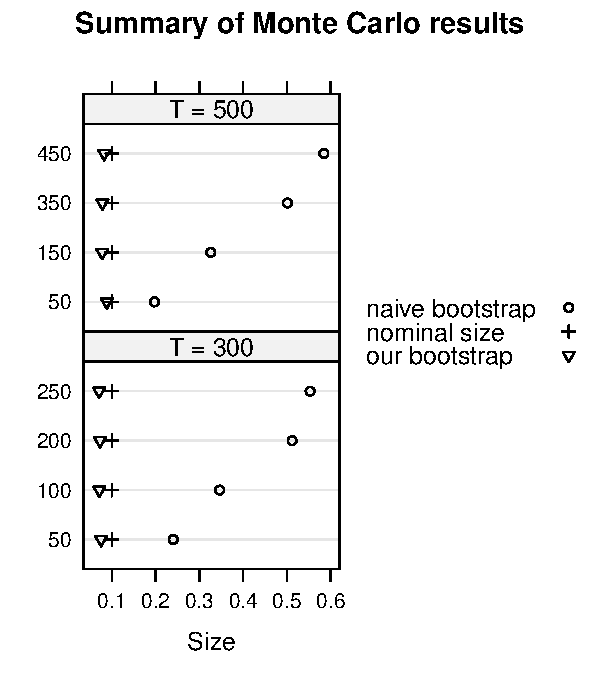
\includegraphics{montecarlo/west_iv.pdf}
  \caption{Results of the Monte Carlo experiment, based on 2000
    simulations from the \dgp described in Section~\ref{sec:mc} with 499
    bootstrap replications each. The circles labeled ``naive bootstrap'' plot the
    actual size
    using resamples of the observed out-of-sample loss to produce the
    bootstrap critical values and the points labeled ``our bootstrap'' use
    the method proposed in this paper. The tests' nominal size is plotted
    for reference.}
  \label{fig:1}
\end{figure}

These results are extremely preliminary and incomplete. For future
versions of the paper we plan to include the following as well:
\begin{itemize}
\item Comparison to \citepos{Wes:96} critical values that do not use
  the bootstrap.
\item Compare studentized statistics (which we don't cover) with
  unstudentized.
\item Use the \dgp\ and statistics from the empirical section to make
  sure that the bootstrap works in that setting and to compare to
  other bootstrap methods.
\item Check \fwe\ control in multiple testing.
\end{itemize}

\section{Conclusion}\label{sec:4}
This paper establishes that standard block bootstraps can be used to
consistently estimate the distribution of asymptotically normal \oos\
statistics. We also show how the bootstrap can be used to correct for
multiple testing in empirical applications, along the lines of
\citepos{Whi:00} Reality Check and provide simulation evidence on the
performance of our approximation in finite samples.

\appendix
\section*{Appendix: Additional mathematical results}\label{sec:B}
\renewcommand{\thesubsection}{\Alph{subsection}}

We will prove our results under the simplifying assumption that there
is a single model and a single sequence of $M$-estimators $\bh_t$. Since we are assuming
non-degeneracy of the models, this assumption does not appreciably
change our arguments. This also implies that we will drop the $i$
index for the estimators $\bh_{it}$, estimation criteria
$q_{it}(\beta)$ etc.

We will also present proofs for the recursive window; the fixed and
rolling window have similar proofs but are less complicated.

To make the mathematical results in this appendix clearer, we will
introduce the following additional notation:
\begin{itemize}
\item $f_t = f_t(\btrue)$ and $f_t^* = f_t^*(\btrue^*)$
\item $F_t(\beta) = \nabla f_t(\beta)$ and $F_t^*(\beta) = \nabla
  f_t^*(\beta)$,
\item $F_t = F_t(\beta_0)$ and $F_t^* = F_t^*(\beta_1^*)$,
\item $F = \E F_t$ and $F^* = \E^* F_t^*$,
\item $h_t(\beta) = \nabla q_t(\beta)$ and $h_t^*(\beta) = \nabla q_t^*(\beta)$,
\item $h_t = h_t(\btrue)$ and $h_t^* = h_t^*(\btrue^*)$.
\end{itemize}
Where it is feasible, we will reuse notation from \cite{Wes:96} and
\cite{WeM:98}.

Also define
\begin{align*}
  S_{ff} &= \sum_{j=-\infty}^\infty \E f_t f_{t-j}' \\
  S_{fh} &= \sum_{j=-\infty}^\infty \E f_t h_{t-j}' \\
  S_{hh} &= \sum_{j=-\infty}^\infty \E h_t h_{t-j}',
\end{align*}
$\pi = \lim P/R$, and
\begin{align*}
  \lambda_{fh} &=
  \begin{cases}
    1 - \pi^{-1} \ln(1 + \pi) & \text{recursive window}, \pi \in (0, \infty) \\
    \pi / 2 & \text{rolling window}, \pi \leq 1 \\
    1 - \pi / 2 & \text{rolling window}, \pi > 1 \\
    0 & \text{fixed window},
  \end{cases} \\
  \lambda_{hh} &=
  \begin{cases}
    2 \lambda_{fh} & \text{recursive window} \\
    \pi - \pi^2/3 & \text{rolling window}, \pi \leq 1 \\
    \pi - 1/3\pi & \text{rolling window} , \pi > 1 \\
    \pi & \text{fixed window}
  \end{cases}
\end{align*}
and define the weights
\begin{equation}\label{eq:1}
  a_t =
  \begin{cases}
    \sum_{s=\max(R-1, t)}^{T-1} 1/s & \text{recursive window} \\
    \min(\tfrac{t}{R-1}, \tfrac{T - t}{R-1}, 1) & \text{rolling window} \\
    \tfrac{P}{R-1} 1\{t < R-1\} &  \text{fixed window}.
  \end{cases}
\end{equation}

Also define $u_1,\dots,u_J$ to be the first period of each
block of the circular bootstrap, and, for each $j = 1,\dots,J$,
define the $\sigma$-fields
\[
\Hs_j = \sigma(u_1,\dots,u_j)
\]
and
\[
\Hs_j^* = \sigma(u_1,\dots,u_j; y_1,\dots,y_T; x_1,\dots,x_T).
\]
Also let $l = T - J \ell$ be the number of elements in the last block.

Finally, for any two $k-$vectors $w$ and $z$, define the $\rect$
operation as the rectangle defined by their elements:
\begin{multline*}
  \rect(w, z) = [\min(w_1, z_1), \max(w_1, z_1)] \times
  [\min(w_2, z_2), \max(w_2, z_2)] \times \cdots \\ \times
  [\min(w_k, z_k), \max(w_k, z_k)].
\end{multline*}

\newcommand{\WesA}[1][]{\oclt{t}
  (F_t^{#1} - \E^{#1} F_t^{#1}) B^{#1} H_t^{#1}}
\newcommand{\WesB}[1][]{\tfrac{1}{\sqrt{P}} \E^{#1} F_t^{#1} \osum{t} (B_t^{#1} -
  B^{#1}) H_t^{#1}}
\newcommand{\WesC}[1][]{\oclt{t}
  (F_t^{#1} - \E^{#1} F_t^{#1}) (B_t^{#1} - B^{#1}) H_t^{#1}}

\subsection*{Proof of Theorem~\ref{T1}}

First, observe that
\begin{equation}\label{eq:24}
  \pr[\sqrt{P} (\fb - \E f_t) \leq x] \to^p \Phi(x / \sigma)
\end{equation}
under our assumptions, which can be shown using arguments directly
following West's (1996).\footnote{%
  Supporting Lemmas presented in this paper's appendix establish the
  intermediate results necessary for the main steps of West's proofs
  to hold under Theorem~\ref{T1}'s assumptions.} %
The scale parameter~$\sigma$ is the asymptotic variance of $\fb$ and
$\Phi$ is the \cdf\ of the standard normal. The conclusion of
Theorem~\ref{T1} then holds if
\begin{equation}\label{eq:23}
  \pr^*[\sqrt{P} (\fb^* - \E^* f_t^*) \leq x] \to^p \Phi(x / \sigma)
\end{equation}
and
\begin{equation}\label{eq:30}
  \var^*(\sqrt{P} \fb^*) \to^p \sigma^2.
\end{equation}
A standard argument attributed to Poly{\`a} ensures that~\eqref{eq:15}
follows from~\eqref{eq:24}--\eqref{eq:30}. (See Chapter 23 of
\citealp{Vaa:00}, for details.)

For~\eqref{eq:23}, begin as in \citet{Wes:96} by expanding
$f_t^{*}(\bh_t^*)$ around $\btrue^*$ to get
  \begin{align*}
    \sqrt{P} (\fb^* - \E^* f_t^*)
    &= \oclt{t} (f_t^{*} - \E^* f_t^*)
     + \oclt{t} F_t^* \cdot (\bh_t^* - \btrue^*)
     + \oclt{t} w_t^* \\
    &= \oclt{t} (f_t^{*} - \E^* f_t^*)
     + F^* B^* \tfrac{1}{\sqrt{P}} \sum_{t=1}^{T-1} a_t h_t^* + o_{p^*}(1)
  \end{align*}
  where
  \begin{equation*}
    w_{t} = \tfrac12 (\bh_t^* - \btrue^*)' \nabla^2 f_{t}^*(b_{t}) (\bh_t^* - \btrue^*),
  \end{equation*}
  and $b_t \in \rect(\bh_t^*, \btrue^*)$ almost surely. The second
  equality holds because $\oclt{t} w_t^* = o_{p^*}(1)$ and
  \begin{equation*}
    \oclt{t} F_t^* \cdot (\bh_t^* - \btrue^*)
    = F^* B^* \tfrac{1}{\sqrt{P}} \sum_{t=1}^{T-1} a_t h_t^* + o_{p^*}(1),
  \end{equation*}
  by Lemma~\ref{SA4}. Lemma~\ref{SA6} implies
  \begin{equation}\label{eq:19}
    \tfrac{1}{\sqrt{P}} \sum_{t=1}^{T-1} \begin{pmatrix}
      (f_t^* - \E^* f_t^*) 1\{t \geq R\} \\ a_t h_t^*
    \end{pmatrix} \to^{d^*}
    N\!
    \begin{pmatrix}
      \begin{pmatrix} 0 \\ 0 \end{pmatrix},
      \begin{pmatrix}
        S_{ff} & \lambda_{fh} S_{fh} \\
        \lambda_{fh} S_{fh}' &  \lambda_{hh} S_{hh}
      \end{pmatrix}
    \end{pmatrix}
  \end{equation}
  and Lemma~\ref{SA1} implies $F^* \to^p F$ and $B^* \to^p
  B$. Then~\eqref{eq:23} holds with
  \begin{equation*}
    \sigma^2 = S_{ff} + \lambda_{fh} (F B S_{fh} + S_{fh}' B'F') + \lambda_{hh} F B S_{hh} B' F'.
  \end{equation*}
  Finally,~\eqref{eq:30} follows from Lemma~\ref{SA5}, completing the
  proof.\qed

\subsection{Supporting Results}

\begin{lema}\label{SA1}
  Under the conditions of Theorem~\ref{T1}, $\btrue^* \to^p
  \btrue$, $B^* \to^p B$, and $F^* \to^p F$.
\end{lema}

\begin{proof}[Proof of Lemma~\ref{SA1}]
  We'll present proofs of these results for the circular block
  bootstrap; the proofs for the moving blocks and stationary
  bootstraps are similar.

  By construction, $\btrue^* = \argmin_\beta \sum_{s=2}^T q_s(\beta)$
  almost surely and our smoothness and moment conditions ensure that
  $\sum_{s=2}^T q_s(\beta)$ obeys a uniform \lln\ and converges in
  probability to $\E q_s(\beta)$ for all $\beta \in \Theta$.
  Consistency of $\btrue^*$ then follows standard arguments; see
  Theorem~2.1 of \cite{NeM:94}, for example.

  For $F^*$, let $\varepsilon$ be an arbitrary positive constant and
  choose $\Delta$ such that $|\beta_1 - \beta_2| < \Delta$ implies
  that $|F(\beta_1) - F(\beta_2) | < \epsilon$ for any $\beta_1$ and
  $\beta_2$ in $N$. Then
  \begin{multline*}
    \pr[|F^* - F| > \epsilon] \leq \\
    \pr[|F^* - F(\btrue^*)| 1\{\btrue^* \in N\} > \epsilon]
      + \pr[\lvert \btrue^* - \btrue \rvert \geq \Delta]
      + \pr[\btrue^* \notin N].
  \end{multline*}
  The second and third probabilities converge to zero since
  $\btrue^* \to^p \btrue$ and the first converges by the uniform
  \lln. The proof for $B^*$ is similar.
\end{proof}

\begin{lema}\label{SA2}
  Under the conditions of Theorem~\ref{T1},
  \begin{gather}
    \omax{t} | \hat{\beta}_{t} - \btrue | \to^{p} 0 \label{eq:26} \\
    \omax{t}  | \hat{\beta}^{*}_{t} - \btrue^* | \to^{p^{*}} 0 \label{eq:27} \\
    \omax{t} \max_{b_t \in \rect(\btrue, \bh_t)}
    \big\lvert - \tfrac{1}{t-1} \sum_{s=1}^{t-1}
    \nabla h_s(b_t) - B^{-1} \big\rvert \to^p 0 \label{eq:21}
    \intertext{and}
    \omax{t}  \max_{b_t \in \rect(\btrue^*, \bh_t^*)}
    \big\lvert -\tfrac{1}{t-1} \sum_{s=1}^{t-1}
    \nabla h_s^*(b_t) - B^{*-1} \big\rvert \to^p 0. \label{eq:22}
  \end{gather}
\end{lema}

The proofs of~\eqref{eq:26} and~\eqref{eq:21} follow standard
arguments and are omitted.

\begin{proof}[Proof of~\eqref{eq:27}]
  For any $\beta \in N$ and $\delta \in (0,1)$,
  \begin{multline}\label{eq:28}
    \tfrac{1}{\delta(T-1)} \sum_{s=1}^{\lfloor \delta(T-1) \rfloor}
    (q_s^*(\beta) - \E^*q_s^*(\beta))
    =  \tfrac{1}{\delta(T-1)} \sum_{j=1}^{\lfloor J_{\delta(T-1)} \rfloor - 1}
    \sum_{s=\ell (j-1) + 1}^{\ell j}
    (q_s^*(\beta) - \E^*_{\ell (j-1)}  q_s^*(\beta)) \\
    + \tfrac{1}{\delta(T-1)} \sum_{s=\ell J_{\delta(T-1)} - \ell + 1}^{\lfloor \delta(T-1) \rfloor}
    (q_s^*(\beta) - \E^*_{\ell (j-1)}  q_s^*(\beta)).
  \end{multline}
  The terms of the outer summation, indexed by $j$, along with the
  last summation considered as a single block, form a Martingale
  Difference Sequence with finite $r$th moments, so it converges in
  probability to zero by the LLN. Stochastic equicontinuity for
  $\beta \in N$ holds because the derivative of $q_s$ has bounded
  $r$th moments for $r > 2$ by assumption and stochastic
  equicontinuity in $\delta$ follows the arguments used in Theorem 2
  of \citet{Cal:14}.

  The remainder of the proof follows the usual steps. \citep[See, for
  example,][]{NeM:94} Take $\varepsilon > 0$ and let
  \[
    \varepsilon' =
    \inf_{\beta : \lvert \beta - \btrue^* \rvert \geq \varepsilon,\ \beta \in N}
    \E^* q_s^*(\beta) - \E^* q_s^*(\btrue^*).
  \]
  Also define $Q^*(b) = \E^* q_s^*(b)$ and
  \[
    \hat t^* = \argmax_{t=R,\dots,T-1} \lvert \bh_t^* - \btrue^* \rvert.
  \]
  Then
  \begin{align*}
    \pr[ \max_{t=R,\dots,T-1} &\lvert \bh_t^* - \btrue^* \rvert > \varepsilon ] \\
    &\leq \pr[ Q^*(\bh_{\hat t^*}^*) > Q^*(\btrue^*) + \varepsilon'
      \text{\ and\ } \btrue^* \in N] + \pr[\btrue^* \notin N] \\
    &\leq \pr\Big[ Q^*(\bh_{\hat t^*}^*) >
     \tfrac{1}{\hat t^*-1} \sum_{s=1}^{\hat t^*-1} q_s^*(\bh_{\hat t^*}^*) + \varepsilon'/3
     \text{\ and\ } \btrue^* \in N\Big] \\
    &\quad+ \pr\Big[ \tfrac{1}{\hat t^*-1} \sum_{s=1}^{\hat t^*-1} q_s^*(\bh_{\hat t^*}^*) >
      \tfrac{1}{\hat t^*-1} \sum_{s=1}^{\hat t^*-1} q_s^*(\btrue^*) + \varepsilon'/3
      \text{\ and\ } \btrue^* \in N\Big] \\
    &\quad+ \pr\Big[\tfrac{1}{\hat t^*-1} \sum_{s=1}^{\hat t^*-1} q_s^*(\btrue^*) >
      Q^*(\btrue^*) + \varepsilon'/3 \text{\ and\ } \btrue^* \in N\Big] \\
    &\quad+ \pr[\btrue^* \notin N].
  \end{align*}
  The first three probabilities converge to zero as a consequence of
  stochastic equicontinuity and the last from consistency of
  $\btrue^*$.
\end{proof}

\begin{proof}[Proof of \eqref{eq:22}.]
For any $\varepsilon$,
\begin{align*}\label{eq:18}
  \pr\Big[&\sup_{t = R,\dots,T-1} \max_{b_t \in \rect(\btrue^*, \bh_t^*)}
  \big\lvert - \tfrac{1}{t-1} \sum_{s=1}^{t-1}
  \nabla h_s^*(b_t) - B^{*-1} \big\rvert > \varepsilon \Big] \\
  &\leq \pr\Big[\sup_{t=R,\dots,T-1}
  \big\lvert - \tfrac{1}{t-1} \sum_{s=1}^{t-1} \nabla h_s^* - B^{*-1} \big\rvert
  1\{\beta_0^* \in N\}> \varepsilon \Big] \\
  &\quad + \pr\Big[\sup_{t=R,\dots,T-1} \max_{b_t \in \rect(\btrue^*, \bh_t^*)}
  \big\lvert - \tfrac{1}{t-1} \sum_{s=1}^{t-1} (\nabla h_s^*(b_t) - \nabla h_s^*)
  \big\rvert 1\{\beta_0^*, \bh_t^* \in N\} > \varepsilon \Big] \\
  &\quad + \pr[\beta_0^* \notin N]
  + \pr[\bh_t^* \notin N \text{\ for some\ } t = R,\dots,T-1].
\end{align*}
The last two probabilities converges to zero by Lemma~\ref{SA1}
and~\eqref{eq:27}.  Moreover, just as in the proof of
Theorem~\ref{T1}, $(1/(t-1)) \sum_{s=1}^{t-1} \nabla h_s^*$ can be is
the sum of a uniformly integrable \mds\ and obeys a uniform \lln, so
\begin{equation*}
  \sup_{t=R,\dots,T-1}
  \big\lvert - \tfrac{1}{t-1} \sum_{s=1}^{t-1} \nabla h_s^* - B^{*-1} \big\rvert
  1\{\beta_0^* \in N\} \to^p 0.
\end{equation*}

It remains to prove
\begin{equation}\label{eq:31}
  \sup_{t=R,\dots,T-1} \max_{b_t \in \rect(\btrue^*, \bh_t^*)}
  \big\lvert - \tfrac{1}{t-1} \sum_{s=1}^{t-1} (\nabla h_s^*(b_t) - \nabla h_s^*)
  \big\rvert 1\{\beta_0^*, \bh_t^* \in N\} \to^p 0.
\end{equation}
Since $\nabla h_s(\beta)$ is continuous uniformly in $N$, choose
$\delta$ so that $|\beta_1 - \beta_2| < \delta$ implies that
$|\nabla h_s(\beta_1) - \nabla h_s(\beta_2)| < \varepsilon$. Then
\begin{multline*}
  \pr\Big[\sup_{t=R,\dots,T-1} \max_{b_t \in \rect(\btrue^*, \bh_t^*)}
  \big\lvert - \tfrac{1}{t} \sum_{s=1}^t
  (\nabla h_s^*(b_t^*) - \nabla h_s^*) \big\rvert 1\{\beta_0^*, \bh_t^* \in N\}
  > \varepsilon \Big]
  \\ \leq \pr[\sup_{t=R,\dots,T-1} \max_{b_t \in \rect(\btrue^*, \bh_t^*)}
  \lvert b_t^* - \btrue^* \rvert > \delta]
\end{multline*}
which converges to zero in probability by~\eqref{eq:27}.
\end{proof}

\begin{lema}\label{SA3}
  If $a \in [0,1/2)$ and the conditions of Theorem~\ref{T1}
  hold, then
  \begin{gather}
    \omax{t} \big\lvert (t-1)^{a-1} \sum_{s=1}^{t-1} h_s \big\rvert \to^p 0 \label{eq:6}\\
    \omax{t} \big\lvert (t-1)^{a-1} \sum_{s=1}^{t-1} h_s^* \big\rvert \to^{p^{*}} 0 \label{eq:11}\\
    \omax{t} (t-1)^a | \hat{\beta}_{t} - \btrue | \to^{p} 0 \label{eq:12} \\
    \omax{t} (t-1)^a | \hat{\beta}^{*}_{t} - \btrue^* | \to^{p^{*}} 0 \label{eq:13} \\
    \oclt{t} \big\lvert \tfrac{1}{t-1} \sum_{s=1}^{t-1} h_s^* \big\rvert = O_{p^*}(1)\label{eq:33}
    \intertext{and}
    \tfrac{1}{\sqrt{P}} \osum{t} (F_t^* - F^*) / (t-1)^a \to^{p^*} 0. \label{eq:32}
  \end{gather}
\end{lema}

\noindent%
The proofs of~\eqref{eq:6} and~\eqref{eq:12} follow similar arguments
to~\citet{Wes:96} and are omitted. Note that~\eqref{eq:12}
and~\eqref{eq:13} are refinements of~\eqref{eq:26} and~\eqref{eq:27}
that adds additional details on the rates of convergence.
All of these proofs will be presented for the case where $h_t$ is
univariate to minimize notational clutter.

\begin{proof}[Proof of~\eqref{eq:11}.]
Let $\delta$ be a positive number less than $1/2 - a$ and define
\[
  H_i^* = (t-1)^{\delta - 1} \sum_{t=K_{i-1}+1}^{K_i} h_t^*,
\] so
\begin{multline}\label{eq:2}
  \omax{t} \big| \tfrac{1}{t-1} \sum_{s=1}^{t-1} h_t^* \big| \leq \\
  R^{-\delta} \max_{j=j^*_R,\dots,J} \big| \sum_{i=1}^{j} H_i^* \big|
  + R^{-\delta} \omax{t} \big| (t-1)^{\delta-1} \sum_{s=K_{j^*_{t - 1}}+1}^{t-1} h_s^* \big|,
\end{multline}
where $j_s^*$ is defined to be the index of the block containing
observation $s$ of the bootstrap sequence.  (So, for example, $j_1^* =
1$.) Now observe that $\{H_i^*, \Hs_i^*\}$ is a martingale difference
sequence, so the maximal inequality implies that
\begin{equation*}
  \pr^*\Big[ \max_{j=j^*_R,\dots,J} \big| \sum_{i=1}^{j} H_{i}^* \big| > \epsilon \Big]
  \leq (1/\epsilon^2) \sum_{i=1}^J \E^*(H_{i}^{*2} \mid \Hs_{i-1}^*).
\end{equation*}
By definition,
\begin{align*}
  \E^*(H_i^{*2} \mid \Hs_{i-1}^*)
  &= \tfrac{1}{T-1} \sum_{u = 0}^{T-2}
  \Big[\sum_{t = 1}^{\ell} h_{u + t}(\btrue^*) / (K_{i-1} + t)^{1-\delta} \Big]^2 \\
  &= \tfrac{1}{T-1} \sum_{u = 0}^{T-2} \Big[\sum_{t = 1}^{\ell}
  (h_{u + t} + h_{u + t}(\btrue^*) - h_{u + t})/ (K_{i-1} + t)^{1-\delta}\Big]^2
\end{align*}
so~\eqref{eq:11} follows from~\eqref{eq:2} combined with
\begin{gather}
  \tfrac{1}{T-1} \sum_{u = 0}^{T-2} \sum_{i=1}^J \Big[\sum_{t = 1}^{\ell}
  h_{u + t}/ (K_{i-1} + t)^{1-a-\delta} \Big]^2 = O_p(1) \label{eq:4} \\
  \tfrac{1}{T-1} \sum_{u = 0}^{T-2} \sum_{i=1}^J
  \sum_{t = 1}^{\ell} \big[(h_{u + t}(\btrue^*) - h_{u + t}) / (K_{i-1} + t)^{1-a-\delta}\big]^2 = O_p(1)
  \label{eq:5}
  \intertext{and}
  \omax{t} \big| \sum_{s=K_{j^*_{t - 1}}+1}^{t-1} h_s^*/(t-1)^{1-a-\delta} \big| = O_{p}(1)\label{eq:14}
\end{gather}
since $R^{-\delta} \to 0$. To establish \eqref{eq:4}, \eqref{eq:5},
and~\eqref{eq:14}, we will exploit the fact that $h_t$ is an
$L_2$-mixingale of size $-1/2$ under our assumptions. Moreover,
$h_t/t^{1-a-\delta}$ is also an $L_2$-mixingale of size $-1/2$ with
constants $c_t/t^{1-a-\delta}$ where $c_t$ and $\zeta_j$ denote the
mixingale constants and coefficients of $h_t$.

First, we show that~\eqref{eq:14} is implied by~\eqref{eq:4}
and~\eqref{eq:5}. Note that
\begin{align*}
  \E^* \big(\omax{t} &\big|\sum_{s=K_{j^*_t - 1}+1}^t h_s^*/(t-1)^{1-a-\delta} \big|\big)^2 \\
  &\leq \E^* \sum_{i=1}^{J} \max_{t = K_{i-1}+1,\dots,K_i} \big| \sum_{s=K_{i-1}+1}^t h_s^*/(t-1)^{1-a-\delta} \big|^2 \\
  &= O_p\Big(\tfrac{1}{T-1} \sum_{i=1}^{J} \sum_{u=0}^{T-2} \max_{t = K_{i-1}+1,\dots,K_i} \big| \sum_{s=K_{i-1}+1}^t h_{s+u} /(t-1)^{1-a-\delta} \big|^2 \\
  &\quad+ \tfrac{1}{T-1} \sum_{i=1}^{J} \sum_{u=0}^{T-2} \max_{t = K_{i-1}+1,\dots,K_i} \big| \sum_{s=K_{i-1}+1}^t (h_{s+u}(\btrue^*) - h_{s+u}) /(t-1)^{1-a-\delta} \big|^2\Big).
\end{align*}
\citepos{Mcl:75} maximal inequality for mixingales implies that
\begin{equation*}
  \E \max_{t = K_{i-1}+1,\dots,K_i} \big| \sum_{s=K_{i-1}+1}^t h_{s+u} /(t-1)^{1-a-\delta} \big|^2
  \leq \E \big| \sum_{s=K_{i-1}+1}^{K_i} h_{s+u} /(s-1)^{1-a-\delta} \big|^2
\end{equation*}
which is the quantity bounded in~\eqref{eq:4}. In addition,
\begin{multline*}
  \tfrac{1}{T-1} \sum_{i=1}^{J} \sum_{u=0}^{T-2} \max_{t = K_{i-1}+1,\dots,K_i} \big| \sum_{s=K_{i-1}+1}^t (h_{s+u}(\btrue^*) - h_{s+u}) /(t-1)^{1-a-\delta} \big|^2 \\
  \leq \tfrac{1}{T-1} \sum_{i=1}^{J} \sum_{u=0}^{T-2} \sum_{s=K_{i-1}+1}^{K_i} \big[(h_{s+u}(\btrue^*) - h_{s+u})/(t-1)^{1-a-\delta}\big]^2,
\end{multline*}
the quantity bounded in~\eqref{eq:5}.

We'll prove~\eqref{eq:4} next, by proving that the expected value of
the LHS is $O(1)$. Using \citepos{Mcl:75} maximal inequality (again)
implies that
\begin{align*}
  \E\Big|\tfrac{1}{T-1}
  &\sum_{u = 0}^{T-2} \sum_{i=1}^J \Big[\sum_{t = 1}^{\ell} h_{u + t}/ (K_{i-1} + t)^{1-a-\delta}\Big]^2 \Big| \\
  &= \tfrac{1}{T-1} \sum_{u = 0}^{T-2} \sum_{i=1}^J \E \Big[\sum_{t = 1}^{\ell} h_{u + t}(\btrue)/ (K_{i-1} + t)^{1-a-\delta} \Big]^2 \\
  &= O\big(\tfrac{1}{T-1}\big) \sum_{u = 0}^{T-2} \sum_{i=1}^J \sum_{t = 1}^{\ell} (K_{i-1} + t)^{2a + 2\delta-2} \\
  &= O(1) \sum_{t=1}^{T-1} t^{2a+2\delta-2}.
\end{align*}
Since $\delta$ was chosen to ensure that $2a+2\delta-2 < -1$, this
last summation is finite as required.

For~\eqref{eq:5}, expanding $h_{u+t}(\btrue^*)$ around $\btrue$ (when
$\btrue^* \in N$) gives
\begin{align*}
  \tfrac{1}{T-1} & \sum_{u = 0}^{T-2} \sum_{i=1}^J \Big(\sum_{t = 1}^{\ell} (h_{u + t}(\btrue^*) - h_{u + t}(\btrue))/ (K_{i-1} + t)^{1-a-\delta} \Big)^2 \\
  &= \tfrac{1}{T-1} \sum_{u = 0}^{T-2} \sum_{i=1}^J \Big(\sum_{t = 1}^{\ell}
  \nabla h_{u + t}(b_{u+t}) \cdot (\btrue^* - \btrue) / (K_{i-1} + t)^{1-a-\delta}\Big)^2 \\
  &= (\btrue^* - \btrue)' \Big[\tfrac{1}{T-1} \sum_{u = 0}^{T-2} \sum_{i=1}^J \sum_{s,t = 1}^{\ell}
  \big(\tfrac{1}{(K_{i-1} + s) (K_{i-1} + t)}\big)^{1-a-\delta} \nabla h_{u + t}(b_{u+t}) \nabla h_{u + s}(b_{u+s})' \Big] (\btrue^* - \btrue) \\
  &= O_p\big(\tfrac{1}{T^2}\big) \sum_{u = 0}^{T-2} \sum_{i=1}^J \sum_{s,t = 1}^{\ell}
  \big(\tfrac{1}{(K_{i-1} + s) (K_{i-1} + t)}\big)^{1-a-\delta} \nabla h_{u + t}(b_{u+t})' \nabla h_{u + s}(b_{u+s})
\end{align*}
where each $b_{u+t} \in \rect(\btrue^*,\btrue)$ almost surely, and so
\begin{align*}
  \pr\Big[& \tfrac{1}{T-1} \sum_{u = 0}^{T-2} \sum_{i=1}^J
  \Big(\sum_{t = 1}^{\ell} (h_{u + t}(\btrue^*) - h_{u + t})/ (K_{i-1} + t)^{1-a-\delta}\Big)^2 > \varepsilon \Big] \\
  & \leq \pr\Big[ \tfrac{1}{T^2} \sum_{u = 0}^{T-2} \sum_{i=1}^J \sum_{s,t = 1}^{\ell}
  \big\lvert \big(\tfrac{1}{(K_{i-1} + s) (K_{i-1} + t)}\big)^{1-a-\delta}
  \nabla h_{u + t}(b_{u+t})' \nabla h_{u + s}(b_{u+s}) \big\rvert 1\{\btrue^* \in N\} > \varepsilon \Big] \\
  &\quad + \pr[\btrue^* \notin N].
\end{align*}
The second probability, $\pr[\btrue^* \notin N]$, converges to zero by
Lemma~\ref{SA1}. For the first, we have
\begin{align*}
  \E \tfrac{1}{T^2} &\sum_{u = 0}^{T-2} \sum_{i=1}^J \sum_{s,t = 1}^{\ell}
  \big\lvert \big(\tfrac{1}{(K_{i-1} + s) (K_{i-1} + t)}\big)^{1-a-\delta}
  \nabla h_{u + t}(b_{u+t})' \nabla h_{u + s}(b_{u+s}) \big\rvert 1\{\btrue^* \in N\} \\
  &\leq \tfrac{1}{T^2} \sum_{u = 0}^{T-2} \sum_{i=1}^J \sum_{s,t = 1}^{\ell}
  \E \sup_{\beta \in N} \big\lvert \big(\tfrac{1}{(K_{i-1} + s) (K_{i-1} + t)}\big)^{1-a-\delta}
  \nabla h_{u + t}(\beta)' \nabla h_{u + s}(\beta) \big\rvert \\
  &\leq O(\tfrac{1}{T^2}) \sum_{u = 0}^{T-2} \sum_{i=1}^J \sum_{s,t = 1}^{\ell}
  \big(\tfrac{1}{(K_{i-1} + s) (K_{i-1} + t)}\big)^{1-a-\delta} \E | m_{u+t} m_{u+s} | \\
  &\leq O(\tfrac{1}{T^2}) \sum_{u=0}^{T-2} \sum_{i=1}^J \sum_{s = 1}^{\ell} (K_{i-1} + s)^{2a + 2\delta - 2} \E m_{u+s}^2
\end{align*}
where the second inequality holds by assumption and the third follows
from repeated application of the Cauchy-Schwarz inequality. Since $\E
m_{u+s}^2$ is bounded, the large summation is $O(T)$ and this final
term converges to zero, completing the proof.
\end{proof}

\begin{proof}[Proof of~\eqref{eq:13}.]
We have already established that both $\bh_t^*$ and $\btrue^*$
are contained in $N$ for large enough $n$. Then expanding
$h_s^*(\bh_t^*)$ around $\btrue^*$ gives
\begin{equation*}
  \bh_t^* - \btrue^* =
  \Big(- \tfrac{1}{t-1} \sum_{s=1}^{t-1} \nabla h_s^*(b_t) \Big)^{-1}
  \tfrac{1}{t-1} \sum_{s=1}^{t-1} h_s^*
\end{equation*}
with each $b_t \in \rect(\bh_t^*, \btrue^*)$ almost surely. Then
\begin{multline}
  \omax{t} (t-1)^a | \hat{\beta}_t - \btrue |
  \leq \omax{t} \big| (t-1)^{a-1} B^* \sum_{s=1}^{t-1} h_s^* \big| \\
  + \omax{t} \Big| \Big(
  - \tfrac{1}{t-1} \sum_{s=1}^{t-1} \nabla h_s^*(b_t^*) \Big)^{-1} - B^* \Big|
  \times \omax{t} \Big| (t-1)^{a-1} \sum_{s=1}^{t-1} h_s^* \Big|.
\end{multline}
These terms converge to zero in (conditional) probability by~\eqref{eq:11}
and Lemma~\ref{SA2}.
\end{proof}

\begin{proof}[Proof of~\eqref{eq:33}.]
  A similar argument to~\eqref{eq:11} establishes that
  \[
    \oclt{t} \Big(\E^* \big\lvert \tfrac{1}{t-1} \sum_{s=1}^{t-1} h_s^* \big\rvert^2\Big)^{1/2}
    = O_p\Big(\oclt{t} (t-1)^{-1/2} \Big)
  \]
  which is $O_p(1)$ by Lemma A1 of \citet{Wes:96}.
\end{proof}
\begin{proof}[Proof of~\eqref{eq:32}.]
  A similar argument to (\ref{eq:11}) establishes that
  \[
    \E^*\Big(\osum{t} (F_t^* - F^*) / (t-1)^a\Big)^2 = O_p(1) \osum{t} (t-1)^{-2a}
  \]
  and the result then follows from Kronecker's Lemma.
\end{proof}

\begin{lema}\label{SA4}
  Under the conditions of Theorem~\ref{T1},
  \begin{equation}\label{eq:16}
    \oclt{t} (\bh_t^* - \btrue^*)' \nabla^2 f_{it}^*(b_{it}^*) (\bh_t^* - \btrue^*) \to^{p^*} 0
  \end{equation}
  and
  \begin{equation}\label{eq:17}
    \oclt{t} F_t^* \cdot (\bh_t^* - \btrue^*)
    = F^* B^* \tfrac{1}{\sqrt{P}} \sum_{t=1}^{T-1} a_t h_t^* + o_{p^*}(1).
  \end{equation}
\end{lema}

\begin{proof}[Proof of~\eqref{eq:16}]
We have
\begin{align*}
  \pr\Big[& \big|\oclt{t} (\bh_t^* - \btrue^*)' \nabla^2 f_{it}^*(b_{it}^*) (\bh_t^* - \btrue^*) \big| > \epsilon \Big] \\
  &\leq \pr\Big[1\{\btrue^* \in N, \bh_t^* \in N\ \text{for all}\ t\} \big|\oclt{t} (\bh_t^* - \btrue^*)' \nabla^2 f_{it}^*(b_{it}^*) (\bh_t^* - \btrue^*) \big| > \epsilon \Big] \\
  &\quad + \pr[\btrue^* \notin N] + \pr[\bh_t^* \notin N\ \text{for some}\ t = R,\dots,T-1\}
\end{align*}
The second two probabilities on the rhs converge to zero by
Lemma~\ref{SA3} and the random variable inside the first probability is bounded by
\begin{multline*}
  1\{\btrue^* \in N, \bh_t^* \in N\ \text{for all}\ t\}
  \oclt{t} (\bh_t^* - \btrue^*)' \nabla^2 f_{it}^*(b_{it}^*) (\bh_t^* - \btrue^*)
  \\ \leq
  \big(\sup_{t=R,\dots,T-1} |P^{1/4}(\bh_t^* - \btrue^*)|^2\big) \oavg{t}  \nabla^2 f_{it}^*(b_{it}^*) 1\{\btrue^* \in N, \bh_t^* \in N\}.
\end{multline*}
The summation is $O_p(1)$ by assumption and the supremum converges to
zero by using Lemma~\ref{SA3} again.
\end{proof}
\begin{proof}[Proof of~\eqref{eq:17}]
For~\eqref{eq:17}, we have the upper bound
\begin{multline*}
  \big\lvert \oclt{t} \big(F_t^* \cdot (\bh_t^* - \btrue^*) - F^* B^* a_t h_t^*\big) \big\rvert \leq \\
   \sup_{s=R,\dots,T-1} |\bh_s^* - \btrue^*|\; \big\lvert \oclt{t} (F_t^* - F^*) \big\rvert
  + \big\lvert F^* \oclt{t} \big((\bh_t^* - \btrue^*) - B^* a_t h_t^*\big) \big\rvert.
\end{multline*}
The first term converges in conditional probability to zero by
Lemma~\ref{SA3}.

For the second, expand each $\sum_{s=1}^t \nabla q_s^*(\bh_t^*)$
around $\btrue^*$ to get
\begin{equation*}
  \oclt{t} (\bh_t^* - \btrue^*)
  = \oclt{t} \Big[\tfrac{1}{t} \sum_{s=1}^t \nabla^2 q_s^*(b_t^*)\Big]^{-1} \tfrac{1}{t} \sum_{s=1}^t h_s^*
\end{equation*}
where $b_t^*$ is between $\bh_t^*$ and $\btrue^*$. Then
\begin{align*}
  \big\lvert \oclt{t} \big((\bh_t^* - \btrue^*) - B^* a_t h_t^*\big) \big\rvert
  &\leq \sup_{t=R,\dots,T-1} \Big\lvert\Big[\tfrac{1}{t} \sum_{s=1}^t \nabla^2 q_s^*(b_t)\Big]^{-1} - B^*\Big\rvert
  \Big\lvert\oclt{t} \tfrac{1}{t} \sum_{s=1}^t h_s^* \Big\rvert \\
  &= O_{p^*}(1) \sup_{t=R,\dots,T-1} \Big\lvert\Big[\tfrac{1}{t} \sum_{s=1}^t \nabla^2 q_s^*(b_t)\Big]^{-1} - B^*\Big\rvert
\end{align*}
by Lemma~\ref{SA3} and the supremum converges to zero in
probability by Lemma~\ref{SA3} as well.
\end{proof}

\begin{lema}\label{SA5}
  Under the conditions of Theorem~\ref{T1}, \eqref{eq:30} holds.
\end{lema}

\begin{lema}\label{SA6}
  Under the conditions of Theorem~\ref{T1}, \eqref{eq:19} holds.
\end{lema}
\begin{proof}

  We will use arguments very similar to \cite{Cal:14}. Define
  \[
  \zeta_{st}^* = \gamma_1'(f_t^* - \E^* f_t^*) + a_s \gamma_2' h_t^*
  \]
  where $\gamma_1$ and $\gamma_2$ are arbitrary nonzero vectors, and
  also define
  \[
  z_j^* = \tfrac{1}{\sqrt{P}} \sum_{s=(j-1) \ell + 1}^{j\ell} \zeta_s^*
  \]
  and
  \[
  v^{*2} = J \var^*(z_j^*)
  \]
  where $\gamma = (\gamma_1', \gamma_2')'$. By construction, $\E^*
  h_t^* = 0$ almost surely, so $\E(z_j \mid \Hs_{j-1}^*) = 0$ almost
  surely and $\{z_j^*, \Hs_j^*\}$ is a martingale difference sequence.

  From the \mds\ property, we have
  \begin{equation*}
    \sum_{j=1}^J z_j^* / \sqrt{v^*} \to^d N(0, 1)
  \end{equation*}
  as long as the following properties hold:
  \begin{equation}\label{eq:7}
    \sum_{j=1}^J \E^*(z_j^{*2} 1\{z_j^{*2} > \epsilon\} \mid \Hs_{j-1}^*) \to^p 0
  \end{equation}
  and
  \begin{equation}\label{eq:8}
    \pr^*\Big[ \big| \sum_{j=1}^J z_j^{*2}/v^{*2} - 1 \big| > \epsilon\Big] \to^p 0.
  \end{equation}

  For~\eqref{eq:8}, we have the usual bound
  \begin{equation*}
    \pr^*\Big[ \big|\sum_{j=1}^J z_j^{*2}/v^{*2} - 1 \big| > \varepsilon\Big] \leq
    \pr^*\Big[ 1\{\btrue^* \in N\} \big| \sum_{j=1}^J z_j^{*2}/v^{*2} - 1 \big| > \epsilon \Big]
     + \pr^*[ \btrue^* \notin N ]
  \end{equation*}
  and we can rewrite the summation in the first term as
  \begin{equation*}
    1\{\btrue^* \in N\} \Big( \sum_{j=1}^J z_j^{*2}/v^{*2} - 1 \Big)
    =  \sum_{j=1}^J \big(1\{\btrue^* \in N\}z_j^{*2}/v^{*2} -
    \E(1\{\btrue^* \in N\}z_j^{*2}/v^{*2} \mid \Hs_{j-1}^*) \big).
   \end{equation*}
   This term is the sum of a uniformly integrable martingale
   difference sequence and satisfies the \lln\ (i.e.\ Davidson's, 1994,
   Theorem 19.7), and so it converges in (conditional) probability to
   zero.  The second term converges in probability to zero by
   consistency of $\btrue^*$ (Lemma~\ref{SA1}).

   Similarly, \eqref{eq:7} holds if
   \begin{equation*}
     1\{\beta_0^* \in N\} \sum_{j=1}^J \E^*(z_j^{*2} 1\{z_j^{*2} > \epsilon\} \mid \Hs_{j-1}^*) \to 0,
   \end{equation*}
   which holds by uniform integrability of $1\{\beta_0^* \in N\} z_j^{*2}$.

   Finally, since the variance of the bootstrapped statistic can be
   rewritten as a \hac\ variance estimator,
   \begin{equation*}
     v^{*2} \to^p \gamma_1' S_{ff} \gamma_1 + 2 \lambda_{fh} (\gamma_2' S_{fh}' \gamma_1)
     + \lambda_{hh} \gamma_2' S_{hh} \gamma_2
   \end{equation*}
   holds by Theorem 2.2 of \cite{JoD:00}, using West's (1996)
   arguments to handle the $a_s$ terms.
\end{proof}

\bibliography{texextra/references}
\end{document}

%%% Local Variables:
%%% mode: latex
%%% TeX-master: t
%%% TeX-command-extra-options: "-shell-escape"
%%% End:

% LocalWords:  ClW JEL ISI Google GiW Mcc ClM CoS CCS StW IMA GiR WeM fh X'X hh
% LocalWords:  PaT AllRefs isi ima uc sv PeT GoW lm il GoK RoW Econometrica PoR
% LocalWords:  Finan StepM studentizing studentization Whi HuW RSW recentering
% LocalWords:  DiM LiS Kun McCracken lt filtrations GoJR JoD McCracken's Econom
% LocalWords:  Corradi unstudentized studentized fg gg GoJ gcalhoun HLN li PoW
% LocalWords:  Econometricians reestimate PPW resample miscentered AnG eq Helle
% LocalWords:  Bunzel Yu Hsu Pincheira HHK th AtO ik DoH Wolak's Wol stepdown
% LocalWords:  Hsu's iq mk Ames Amit Goyal rfs Ivo Welch Wes covariance MeR McW
% LocalWords:  familywise prespecified CoD Gia pointwise misspecified InK MeP
% LocalWords:  VeR xtable Dah dbframe oos parametrizations iid dgp return's CaT
% LocalWords:  outperformance Hmisc Har nondifferentiable bT jt Meng
% LocalWords:  stationarity mixingale mixingales texextra Timmermann